\begin{figure}[h] 
\centering 
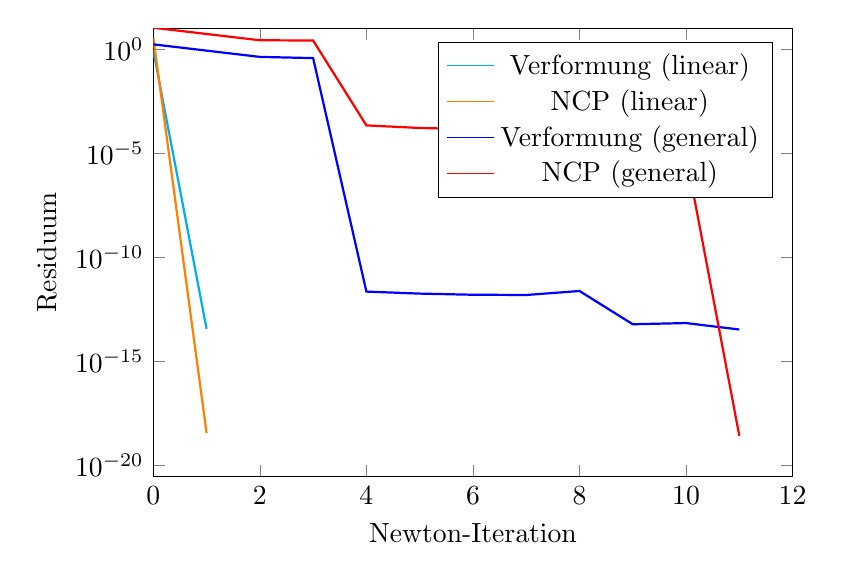
\begin{tikzpicture}[every plot/.append style={thick}] 
\begin{axis}[ 
label style={font=\normalsize}, 
xlabel={Newton-Iteration}, 
ylabel={Residuum}, 
xmin=0, xmax=12, 
ymode=log, 
ymin=0, ymax=10, 
width=0.8\textwidth, 
height=0.6\textwidth, 
legend pos=north east, 
legend style={cells={align=left}}, 
grid style=dashed, 
] 
\addplot[ 
color=cyan, 
] 
coordinates { 
(0, 8.51e-01)(1, 3.60e-14)}; 
\addlegendentry{Verformung (linear)} 
\addplot[ 
color=orange, 
] 
coordinates { 
(0, 3.58e+00)(1, 3.53e-19)}; 
\addlegendentry{NCP (linear)} 
\addplot[ 
color=blue, 
] 
coordinates { 
(0, 1.68e+00)(1, 8.38e-01)(2, 4.19e-01)(3, 3.67e-01)(4, 2.21e-12)(5, 1.77e-12)(6, 1.56e-12)(7, 1.52e-12)(8, 2.36e-12)(9, 5.96e-14)(10, 6.80e-14)(11, 3.33e-14)}; 
\addlegendentry{Verformung (general)} 
\addplot[ 
color=red, 
] 
coordinates { 
(0, 1.06e+01)(1, 5.29e+00)(2, 2.64e+00)(3, 2.57e+00)(4, 2.14e-04)(5, 1.61e-04)(6, 1.41e-04)(7, 1.36e-04)(8, 5.05e-05)(9, 5.13e-05)(10, 8.41e-06)(11, 2.60e-19)}; 
\addlegendentry{NCP (general)} 
\end{axis} 
\end{tikzpicture} 
\caption{Residuen des Stoffgesetzes 'Linear elastisch' mit Hinderniss 'Hut' und 8450 Freiheitsgraden für die Verschiebung.} 
\label{fiq:Linearelastisch_Hut_level5} 
\end{figure} 
